%% Advanced fields & particles final report
%% Topic : YM instantons
%% Author : Seongmin Kim, Taeyoon Kim
%% Date : 2020. 06. 15
%% 폭 넓게 쓰라고
\documentclass{article}
\usepackage{amssymb}
\usepackage{slashed}
\usepackage{hyperref}
\usepackage{tikz}
\usepackage{pgfplots}
\usepackage{subcaption}
\usepackage{tikz-cd}
\usepackage{amsmath}
\usepackage{amsfonts}
\usepackage{graphicx} % Required for inserting images
\usepackage{amsthm}
\usepackage[scr=rsfs]{mathalpha}

\newtheorem{defn}{Definition}
\newtheorem{thm}{Theorem}
\newtheorem{lem}{Lemma}
\newtheorem{prop}{Proposition}
\newtheorem{rem}{Remark}
\newtheorem{note}{Note}
\newtheorem*{exa}{Ex)}

\title{Yang-Mills Instantons}
\author{Seongmin Kim, Taeyoon Kim}
\date{\today}

%% 폭 넓게 하라고
\usepackage{geometry}
\geometry{
    a4paper,
    total={170mm,257mm},
    left=20mm,
    top=20mm,
}

\begin{document}

\maketitle

\section{Introduction : What is an Instanton?}

%% 줄글 형식
%% Instanton is a solution to the classical field equations of motion in Euclidean space.
%% Instanton, a solutions of Euclidean EL equation are localized in (Euclidean) space and time, and have finite (Euclidean) action.
%% One way to understand instantons is to consider them as a way to evaluate tunneling events in the path integral formulation of quantum field theory.
%% Instantons are important in understanding non-perturbative effects and tunneling between vacua in quantum field theory.
%% Instantons only appear in Euclidean space, and they are not solutions to the equations of motion in Minkowski space. So, they are not physical particles or fields, in Real spacetime.
%% 너가 유연하게 introduction을 쓰라고

What is instanton? Instanton is a solution to the classical field equations of motion in Euclidean space. Instanton solutions of Euclidean EL equation are localized in (Euclidean) space and time, and have finite (Euclidean) action. This is why it is called instanton.
Instantons only appear in Euclidean space, and they are not solutions to the equations of motion in Minkowski space. So, they are not physical particles or fields, in Real spacetime. So, why do we care about instantons? 
The answer is that we essentially need wick rotation and Euclidean space to perform path integral calculations in (Minkowski) quantum field theory. 
So even we are interested in Minkowski space, we should consider instantons, which are classical solutions in Euclidean space.
In detail, how do instantons affect the QFT in Minkowski space? We will discuss how the instanton effect appears in the path integral formulation, and how it is related to various physical phenomena. 


\section{Instanton effect in Path Integral : a Toy Model}

%% Instanton effect in path integral
\subsection{$0+1$ Dimensional Toy Model : QM with a double well potential}

Let's consider a simple toy model, a quantum mechanical system with a double well potential. The action of the system is given by
\begin{equation}
    S = \int dt \left( \frac{1}{2} \dot{x}^2 - V(x) \right)
\end{equation}
where the potential is given by $V(x) = \frac{1}{8}(x^2-1)^2$.
The classical vacuum structure of the system is shown in Fig. \ref{fig:doublewell}.
\begin{figure}[h]
    \centering
    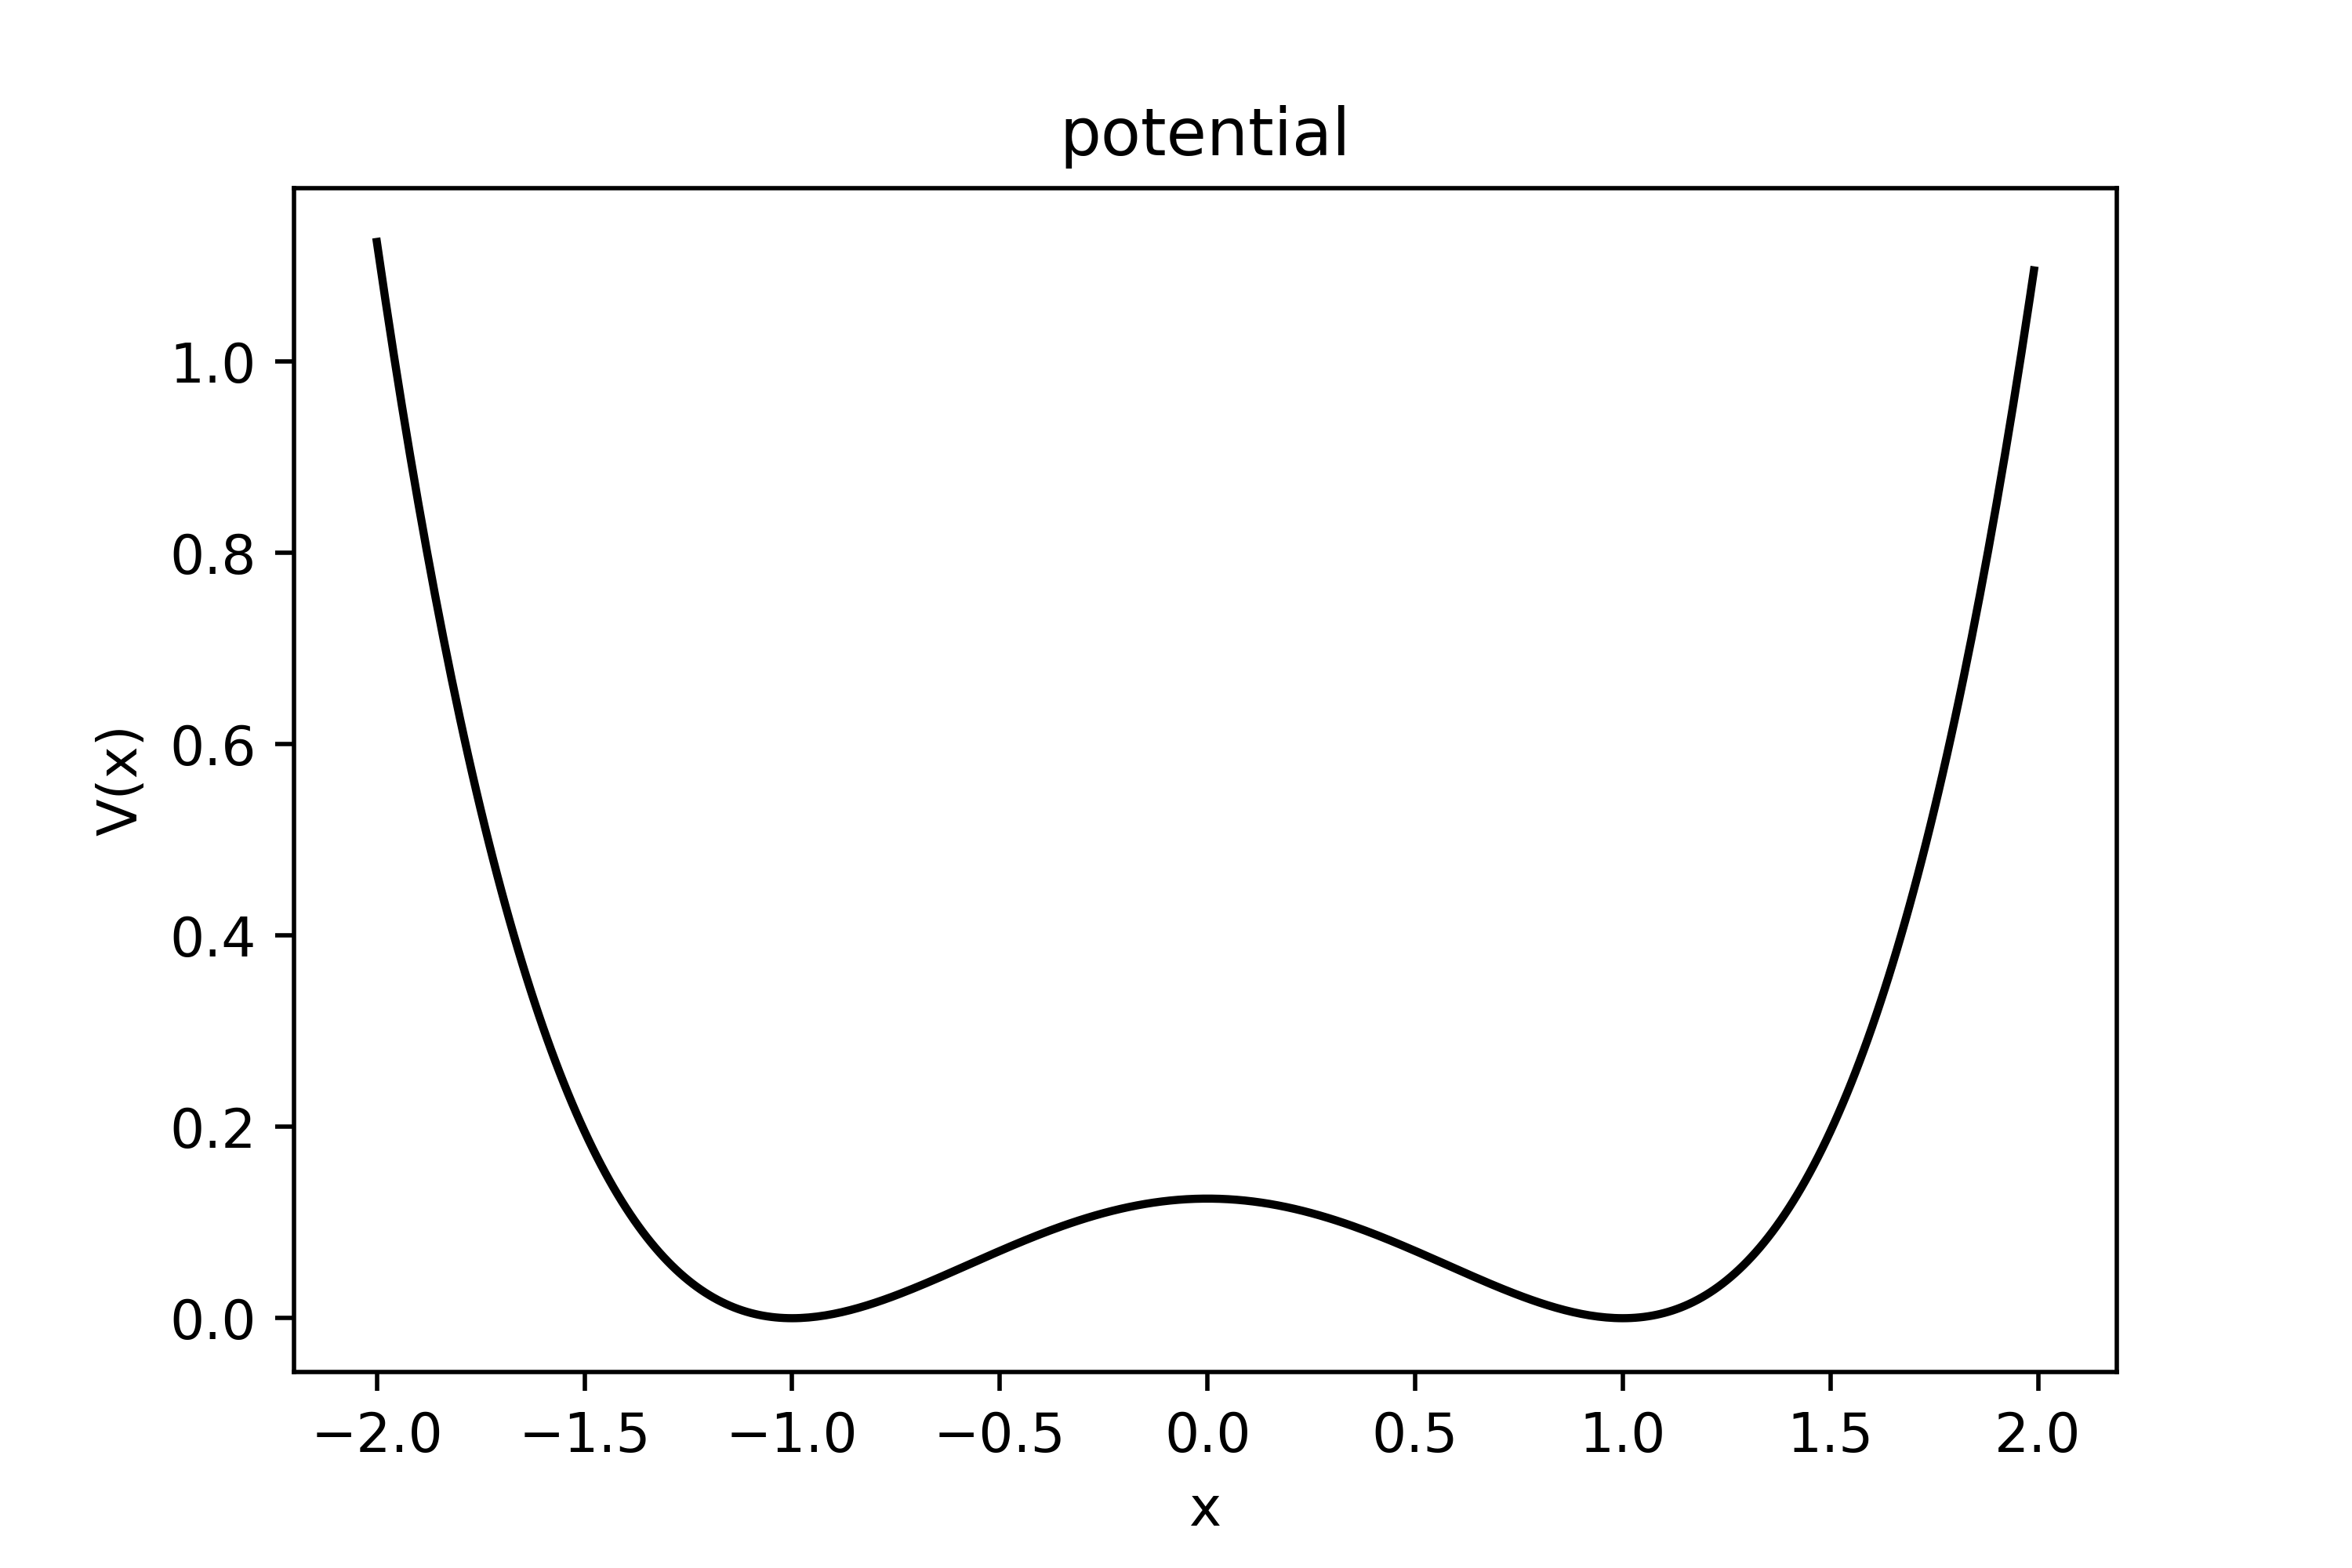
\includegraphics[width=0.5\textwidth]{potential.png}
    \caption{The vacuum structure of the double well potential, there are two minima at $x = \pm 1$.}
    \label{fig:doublewell}
\end{figure}

Classically, the system has two minima at $x = \pm 1$, but quantum mechanically, the system can tunnel between the two minima.
So the true quantum ground state of the system is a superposition of the two classical ground states, and this splitting of the ground state is totally determined by the tunneling amplitude between the two minima.
Now, we will evaluate the tunneling amplitude using the path integral formulation of quantum mechanics, including the instanton solution of the system. 




\subsection{Path Integral Formulation and Wick Rotation}


When we consider the path integral of the system, the path integral is given by $Z = \int \mathcal{D}x e^{iS[x]}$.
But, this integral doesn't converge well, so we need to consider the path integral in Euclidean space, $Z = \int \mathcal{D}x e^{-S_E[x]}$, where $S_E[x] = \int dt \left( \frac{1}{2} \dot{x}^2 + V(x) \right)$.
And to evaluate the original path integral, we just need to wick rotate the time variable, $t \rightarrow -i\tau$.

This looks like just a mathematical trick, and not an essential part of the theory, but in fact, this wick rotation is essential.
Why? There is no way to consider the instanton effect in the path integral formulation in Minkowski space, because the instanton solutions only appear in Euclidean space.
Then, is there any posibility to evaluate the instanton effect in Minkowski space? Like using the perturbative expansion of the path integral? The answer is no. The instanton effect is a non-perturbative effect, and it cannot be evaluated by the perturbative expansion of the path integral.
So, the wick rotation is essential to evaluate the instanton effect in the path integral formulation of quantum field theory.

\subsection{Instanton Solutions in Euclidean Space}


The instanton solution of the system is given by the bounce solution, which is a solution to the Euclidean equation of motion, $\delta S_E = 0$.
The bounce solution is a solution that interpolates between the two minima of the potential, and it is localized in Euclidean time.
Now, we will calculate the bounce solution of the system, and evaluate the instanton action of the bounce solution.

The euclidean Lagrangian is :
\[
    L_E = \frac{1}{2}\dot{x}^2 + \frac{1}{8}(x^2-1)^2
\]

\[
    S_E = \int_{\tau_i}^{\tau_f} L_E d\tau
\]
While the boundary conditions are that $x(-\inf)=-1$, $x(+\inf)=1$. One can observe that action can have a definite minimum, just by a simple calculation :
\[
    S_E = \int_{-\infty}^{\infty} \left(\frac{1}{2} (\dot{x}+\frac{1}{2}(x^2-1))^2 - \frac{1}{2}\frac{dx}{d\tau}(x^2-1) \right)d\tau
\]
\[
    =\int_{-\infty}^{\infty} \left(\frac{1}{2} (\dot{x}+\frac{1}{2}(x^2-1))^2 \right)d\tau - \int_{-\infty}^{\infty}   \frac{1}{2}\frac{dx}{d\tau}(x^2-1) d\tau
\]
\[
    =\int_{-\infty}^{\infty} \frac{1}{2} \left(\dot{x}+\frac{1}{2}(x^2-1)\right)^2 d\tau + \int_{-1}^{1}    dx \  \frac{1}{2}(1-x^2) \geq \int_{-1}^{1}    dx \  \frac{1}{2}(1-x^2) \ = \ \frac{2}{3}
\]
The first term is always non-negative, and can be minimized to 0 by the solution of the EL equation. 
The second term is a constant, and this is the action of the instanton solution.


\[
    \frac{dx}{d\tau} = -\frac{1}{2}(x^2-1)
\]
\[
    \frac{1}{2} (\frac{1}{1-x}+\frac{1}{1+x})dx =\frac{dx}{1-x^2} = \frac{1}{2}d\tau
\]

Hence,
\[
    d\log(\frac{1+x}{1-x}) = d\tau
\]
This can be simplified as the following.
\[
    x(\tau) = \mathrm{tanh}(\frac{1}{2}(\tau-\tau_0))
\]

Which is the solution, ranging over $-\infty$ to $\infty$. This is an absolute minimum, which is also a solution to EOM.

The instanton action is given by $S_{\text{inst}} = \frac{2}{3}$, and the solution is shown in the figure \ref{fig:instanton}.

\begin{figure*}
    \centering
    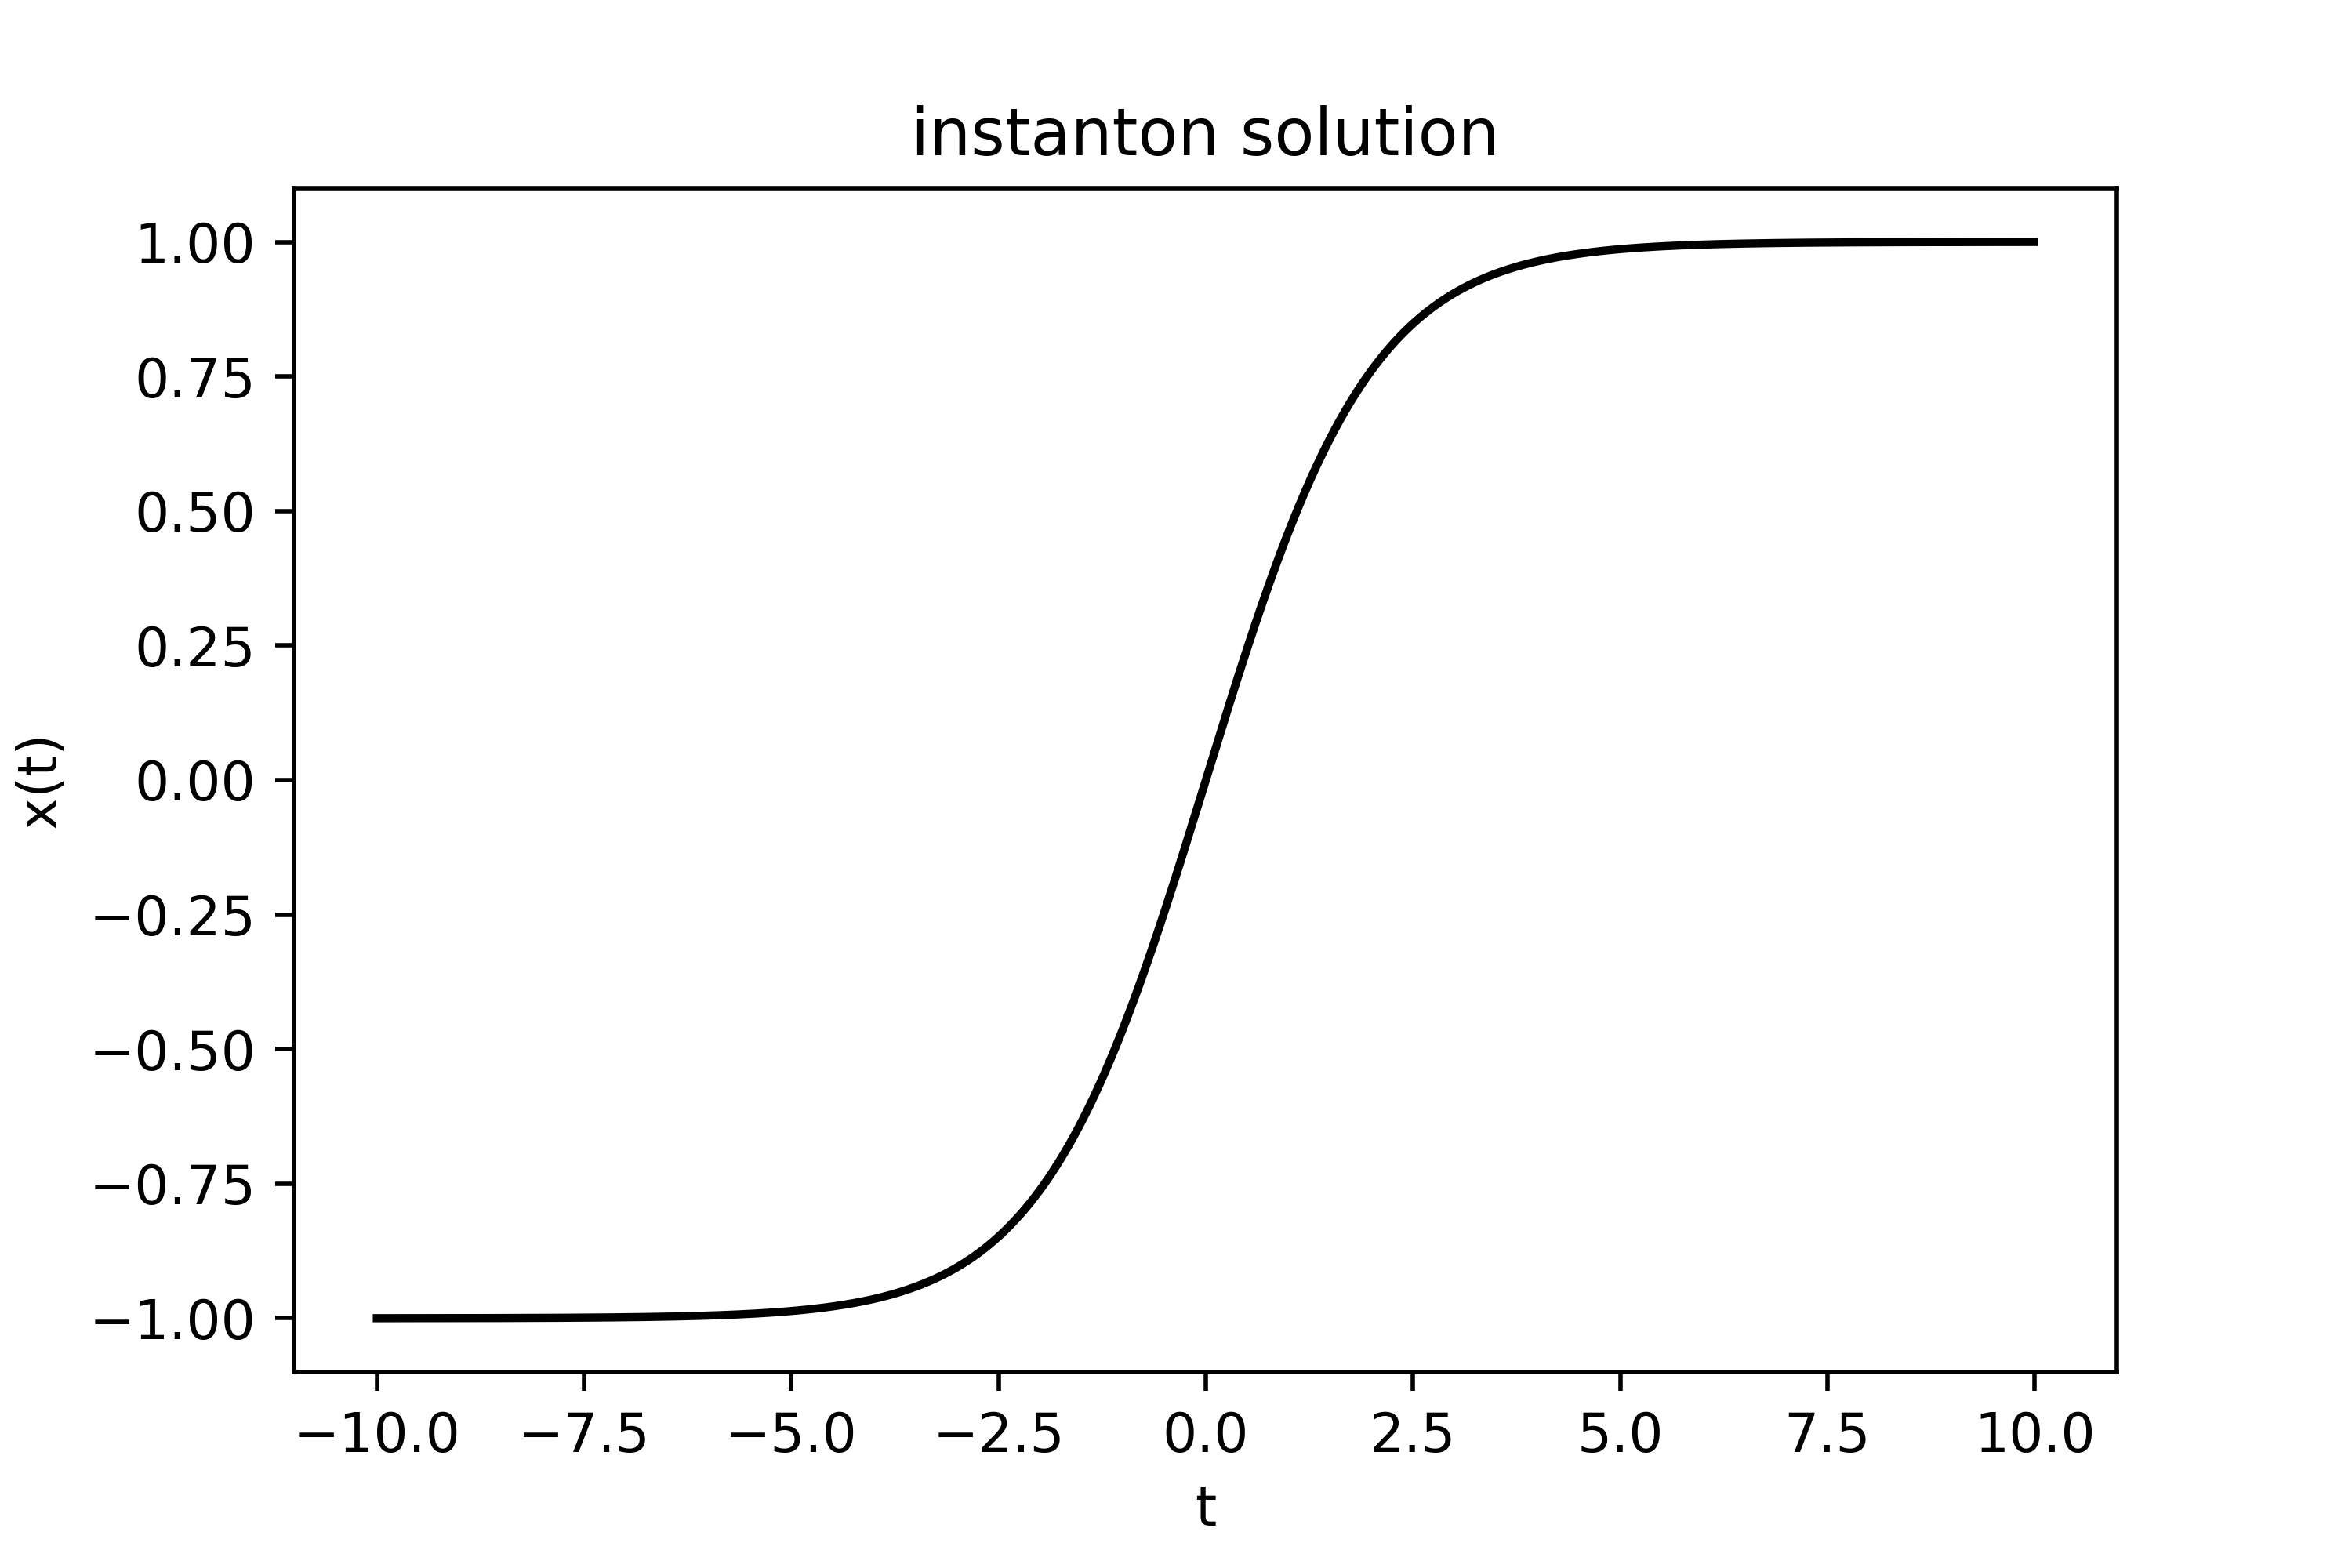
\includegraphics[width=0.5\textwidth]{instanton.png}
    \caption{The instanton solution of the double well potential, which interpolates between the two minima of the potential.}
    \label{fig:instanton}
\end{figure*}



\subsection{Instanton Contribution to the Path Integral}

The path integral of the system is given by the sum of all possible paths. In the semiclassical limit, the path integral is dominated by the classical solutions, (i.e., the instanton solutions) and the small fluctuations around them.
So the full path integral is given by the sum of all instanton contributions, with small fluctuations around them.
\begin{equation}
    Z = \int \mathcal{D}x e^{-S[x]} = \sum_{\text{instantons}} e^{-S_{\text{inst}}} \int \mathcal{D}\delta x e^{-S_{\text{fluct}}[\delta x]}
\end{equation}
where $S_{\text{inst}}$ is the action of the instanton solution, and $S_{\text{fluct}}$ is the action of the small fluctuations around the instanton solution.
This is how the instanton effect appears in the path integral formulation of quantum field theory. Normally, the instanton effect is not easy to calculate, but in this toy model, we can calculate the instanton effect by hand, with the bounce solution.
To evaluate the path integral, we need to consider all the possible classical paths.
Any classical path between the two minima of the potential can be considered as a composition of $n$ single bounce solutions, at time $t_1, ... t_n$, and the instanton action of this classical path is given by $S = \sum_{i=1}^n S_{\text{inst}}=nS_{\text{inst}}$.

So, the Euclidean path integral, from $x = -1$ to $x = 1$, is given by the sum as :
\begin{equation}
    \langle x = 1 | e^{-HT} | x = -1 \rangle = \sum_{n \ \text{odd}} e^{-nS_{\text{inst}}} \int_{0}^T \text{d}t_1 \int_{t_1}^T \text{d}t_2 \cdots \int_{t_{n-1}}^T \text{d}t_n \int \mathcal{D}\delta x e^{-S_{\text{fluct}}}
\end{equation}

The path integral of the fluctuation can be factorized into $n+1$ parts, which are the fluctuation path integrals around each instanton solution, and one for the fluctuation around the classical ground state.
Using this factorization, we can approximated, $\int \mathcal{D}\delta x e^{-S_{\text{fluct}}} \approx \left( \int \mathcal{D}\delta x_0 e^{-S_{\text{fluct}0}} \right)^n e^{-T/2}=K^n e^{-T/2}$
Finaly, we get
\begin{equation}
    \langle x = 1 | e^{-HT} | x = -1 \rangle = e^{-T/2} \sum_{n \ \text{odd}} \frac{T^n}{n!} K^n e^{-nS_{\text{inst}}}= e^{-T/2}  \text{sinh}(KT e^{-S_{\text{inst}}})
\end{equation}

So this is the matrix element of $e^{-HT}$ from $x = -1$ to $x = 1$, using the path integral including instanton solution. 
To evaluate the propagator in Minkowski space, one cas just change the time variable back to Minkowski time, $T \rightarrow -iT$.
Then, the propagator is given by $\langle x = 1 | e^{-itH} | x = -1 \rangle = e^{-it/2}  \text{sin}(Kt e^{-S_{\text{inst}}})$.

\subsection{Tunneling Amplitude, Instanton Action and WKB Approximation}

In Hamiltonian formalism, the oscillatory behavior of the propagator
\begin{equation}
    \langle x = 1 | e^{-itH} | x = -1 \rangle = e^{-it/2}  \text{sin}(Kt e^{-S_{\text{inst}}})
\end{equation}
can be understood as an oscilation due to the tunneling amplitude between the two minima of the potential.


The tunneling amplitude, $\langle x=1 | H | x=-1 \rangle $, can be evaluated with the WKB approximation, which can be evaluated by approximating the shrodinger equation with the WKB wavefunction.

The result is well known. The tunneling amplitude from two classical vacuum with enegry E, from $x = a$ to $x = b$ is generally given by
\begin{equation}
    \langle x = a | H | x = b \rangle \propto \text{exp}\left( -\int_a^b  dx \ \sqrt{2m(V(x)-E)} \right)
\end{equation}

We can easily show that this WKB approximation is equivalent to the path integral result :
    
\begin{align}
    \dot{x}^2&=2(V(x)-E)/m \rightarrow \dot{x} = \sqrt{2(V(x)-E)/m} \\
    S_{\text{inst}} &= \int d\tau \left( \frac{1}{2} m \dot{x}^2 + V(x) \right) = \int d\tau \left( \frac{1}{2} m \dot{x}^2 + \frac{1}{2} m \dot{x}^2 + E   \right) \\
    &= \int dx \ m\dot{x} + E\tau = \int dx \ \sqrt{2m(V(x)-E)} + E\tau 
\end{align}

So the instanton action is the same as the WKB action, and the tunneling amplitude is given by the instanton action, $e^{-S_{\text{inst}}}$.
Instanton is a essential ingredient to evaluate the tunneling amplitude in the path integral formulation, and the same result can be obtained by the WKB approximation.
Here one might wonder, can't we just obtatain the tunneling amplitude by path integral in Minkowski space? Well, the answer is no. We will discuss this in the next section.

\subsection{The non-perturbative behavior of the propagator}
The propagator in the double well potential was calculated as
\begin{equation}
    \langle x = 1 | e^{-itH} | x = -1 \rangle = e^{-it/2}  \text{sin}(Kt e^{-S_{\text{inst}}})
\end{equation}

In this section, we will discuss the non-perturbative behavior of the propagator.
Here, the term "non-perturbative" means that phisical quantities are not analytic in $\hbar$, and cannot be evaluated by the perturbative expansion of the path integral.
So we have to re-introduce $\hbar$ to our calculation, and show that this is not an analytic function of $\hbar$, at $\hbar = 0$.

With $\hbar$, the propagator is given by
\begin{equation}
    \langle x = 1 | e^{-itH/\hbar} | x = -1 \rangle = e^{-it/2}  \text{sin}(Ke^{-S_{\text{inst}}/\hbar} t/\hbar)
\end{equation}

The $e^{-S_{\text{inst}}/\hbar}$ term is non-analytic in $\hbar$, and it is not possible to evaluate this term by the perturbative expansion of the path integral.
This is because the path integral expansion is in fact, the expansion in $\hbar$. This looks unfamiliar because we usually think of the path integral as the expansion in the coupling constant, and we use $\hbar=1$ conventionally.
But in fact, in the feynman diagrams, the order of $\hbar$ is the order of the loop expansion, so the perturbative path integral expansion gives an asymptotic series in $\hbar$.

So if you don't have a brand new idea to evaluate path integral non-perturbatively in Minkowski space, you have to go to the Euclidean space, and consider the instanton solutions to evaluate all the non-perturbative effects.
Going to Euclidean space is not just a mathematical trick, but an essential part of the path integral, in order to overcome the limit of the perturbative expansion of the path integral.
\section{Yang-Mills Instanton}
Now, you have a basic understanding of the instanton effect in the path integral formulation of quantum theory.
Why is it essential, and how does it appear in the path integral, and how does it affect the physical phenomena.
The phisics of Yangs-Mills instanton is not so much different from the toy model we discussed, but the mathematical structure is highly more complicated.
In this section, we will focus on the mathematical structure of the Yang-Mills instanton, and discuss the "moduli space" of the instanton solutions.

\section*{Yang Mills Theory}

\begin{rem}[Exterior Covariant derivative]
    One can define the exterior covariant derivative. 
    \[
        d_\nabla: \Omega^k(M,E)\rightarrow \Omega^{k+1}(M,E)
    \]
    With the following properties. For $s\in \Gamma(M,E)$,
    \[
        d_\nabla s = \nabla s 
    \]
    For $\omega\in \Omega^k(M,E)$, $\eta \in \Omega^l(M,E)$
    \[
        d_\nabla(\omega \wedge \eta ) = d_\nabla \omega \wedge \eta + (-1)^k \omega \wedge d_\nabla \eta
    \]
\end{rem}

Note that this exterior covariant derivative gets along well with our former calculation. 

\begin{note}
    Select a local frame of $E$ as $\{e_1\cdots e_r\}$. 
    $\omega = \sum \omega^i\otimes e_i$, $\omega_i \in \Omega^k(M)$. One can calculate the exterior covariant derivative.
    \[
        d_\nabla \omega = d_\nabla e_i \wedge \omega_i + e_i \otimes d\omega_i = A^j_i e_j \wedge \omega^i + e_i \otimes d\omega^i = e_j \otimes (d\omega^j + A^j_i \wedge \omega^i)
    \]
    For some covariant derivative matrix $A\in\Omega^1(M,\mathrm{End} E)$ for local frames. 
    \[
        d_\nabla \omega = d\omega + A\wedge \omega
    \]
\end{note}

Since it is crucial to calculate covariant derivative for endomorphism valued forms, one needs to define the following covariant derivative. 

\begin{rem}[Covariant Derivative on $\mathrm{End}E$]
    For $\eta\in \Gamma(M,\mathrm{End}E)$, $s\in \Gamma(M,E)$, the covariant derivative of $\eta$ is defined as the following. 
    \[
        \nabla^{\mathrm{End}E}_X(\eta) (s) = \nabla_X^E(\eta s) - \eta \nabla_X^E(s)
    \]
    Which inherits the property of the Leibniz rule. 
\end{rem}

It is valid to define new exterior covariant derivative for endomorphism valued forms. 

\begin{prop}[Exterior Covariant Derivative for Endomorphism]
    Exterior Covariant derivative for endomorphism also must have the following property.
    For $\eta\in\Omega^k(M,\mathrm{End}E)$, $\omega \in \Omega^l(M,E)$,
    \[
        d_\nabla^E(\eta\wedge\omega) = d_\nabla^{\mathrm{End}E}(\eta) \wedge \omega+ (-1)^k \eta\wedge d_\nabla^E(\omega)
    \]
\end{prop}
\begin{proof}
    Rewrite that $\eta = A\otimes \alpha$, $\omega = s \otimes \beta$ For $\alpha,\beta\in\Omega^*(M)$.
    \[
        d_\nabla^E(A(s)\otimes\alpha\wedge\beta) = \nabla^E(A(s))\otimes\alpha\wedge\beta + A(s)d_\nabla^E(\alpha\wedge\beta)
    \]
    \[
        =(\nabla^{\mathrm{End}E}A(s)+A(\nabla^Es))\otimes \alpha \wedge \beta + A(s)(d\alpha\wedge\beta +(-1)^k\alpha\wedge d\beta)
    \]
    \[
        =(\nabla^{\mathrm{End}E}A\wedge\alpha+A\otimes\alpha)\wedge(s\otimes\beta) + (-1)^k(A\otimes\alpha)(\nabla^Es\otimes\beta + s\otimes d\beta)
    \]
    \[
        = d_\nabla^{\mathrm{End}E}(A\otimes\alpha) \wedge s\otimes\beta+ (-1)^k A\otimes \alpha\wedge d_\nabla^E(s\otimes\beta)
    \]
\end{proof}
By this calculation, we can assure that endomorphism valued forms admit exterior covariant derivative. And now we omit the $\mathrm{End}E$ for such symbols. \\
For a vector bundle $E$ over $M$, one can define the Yang-Mills action defined on the space of connections of $E$.

\begin{defn}[Yang-Mills Action] 
\[
    S_{YM}(\nabla) = \int_M \frac{1}{2g^2} \mathrm{tr}(F_\nabla\wedge\star F_\nabla) = \int_M \frac{1}{2g^2} \langle F_\nabla, F_\nabla \rangle \mathrm{Vol}_g
\]
In coordinate basis, 
\[
    S_{YM}(\nabla) = \int_M d^4 x \frac{1}{2g^2} \mathrm{tr}(F^{\mu\nu}F_{\mu \nu})
\] 
While $F$ is endomorphism valued 2 forms on M. 
\end{defn}
More physically, one can make a same description for principal G bundle over M. The associated vector bundle(i.e. its lie algebra bundle) would give the same construction on Yang-Mills Action. It is valid to consider its saddle point, checking classic solutions. This is the natural reason why one has the $\mathrm{tr}$ for the action, since the natural metric for (semi-) simple lie algebra is the Killing form. 

\begin{prop}[Yang-Mills Equation of motion]
     $F$ that lies on the critical point of the action functional satisfies the equation, $d_\nabla^{\star}F=0$, while $d_\nabla^\star$ represents the adjoint of $d_\nabla$. 
\end{prop}
\begin{proof}  
    Consider the following $\nabla_t = \nabla + tA$ for arbitrary $A$. Which yields the t-dependent $F_t = F_\nabla + t d_\nabla A + \frac{t^2}{2} [A,A]$
    \[
        \left. \frac{d}{dt} \right|_{t=0}  S_{YM}(\nabla+tA) = \int_M \frac{1}{g^2} \mathrm{Vol}_g \langle F_\nabla, d_\nabla A\rangle = \int_M \frac{1}{g^2} \mathrm{Vol}_g \langle d_\nabla ^\star F_\nabla, A\rangle =0
    \]

    Giving that $d_\nabla ^\star F = 0$.
\end{proof}


\begin{note}
    One can calculate $d_\nabla d_\nabla \omega$ for $\omega\in\Omega^k(M,E)$.
    \[
        d_\nabla d_\nabla\omega = d_\nabla(d\omega+A\wedge\omega) = d(A\wedge\omega)+A\wedge(d\omega + A\wedge\omega)
    \]
    \[
        =(dA+A\wedge A)\omega = F_\nabla \wedge \omega
    \]
\end{note}


\begin{rem}
    The Bianchi identity, $d_\nabla F = 0$ must be satisfied for any endomorphism valued 2 forms. 
\end{rem}
\begin{proof}
    For any $\omega\in\Omega^1(M,E)$,
    \[
    (d_\nabla)^3\omega = d_\nabla(F_\nabla\wedge\omega) = d_\nabla F_\nabla\wedge\omega + F_\nabla \wedge d_\nabla\omega
    \]
    \[
        =(d_\nabla)^2 d_\nabla\omega = F_\nabla \wedge d_\nabla \omega
    \]

    Therefore we have $d_\nabla F_\nabla=0$
\end{proof}

Through this process, one can derive PDE that $F_\nabla$ must satisfy for classic Yang Mills gauge theory. To simplify, 
\[
    d_\nabla^\star F_\nabla = 0, d_\nabla F_\nabla = 0
\]

\section*{Yang Mills Instanton}

\begin{defn}[Hodge star operator]
    One can define the following Hodge star operator for n-dimensional Riemannian manifold $(M,g)$.
    \[
     \star : \Omega^k(M)\longrightarrow \Omega^{n-k}(M)
    \]
    such that for any $\eta\in \Omega^k(M)$,
    \[
        \langle\eta,\omega\rangle \mathrm{Vol}g =\eta \wedge \star \omega
    \]
    While the $\mathrm{Vol}g$ represents the volume form of the Riemannian manifold $M$.
\end{defn}

\begin{note}[Hodge star operator for index notation]
    Choosing the coordinate chart $(U,\phi = (x^1,\cdots ,x^n))$ for $M$, one can explicitly write down the Hodge star operator for k forms.
    \[
        \star (dx^{i_1}\wedge \cdots \wedge dx^{i_k}) = \frac{\sqrt{\mathrm{det}g_{ij}}}{(n-k)!} g^{i_1 j_1}\cdots g^{i_k j_k} \epsilon_{j_1\cdots j_n} dx^{j_{k+1}}\wedge\cdots\wedge dx^{j_n}
    \]
\end{note}
\begin{note}
    One can calculate the following $\star\star:\Omega^k(M)\rightarrow\Omega^k(M)$.
    And it is known that $\star\star\omega = (-1)^{k(n-k)}\omega$. And for $n=4$, $k=2$, $\star\star = \mathrm{id}$  on $\Omega^2(M)$.
\end{note}
While it is natural to define such star operator on vector valued or endomorphism valued forms, to just apply it on the differential form part. Therefore, one can define the following.
\begin{defn}[Yang Mills Instanton]
    $F\in\Omega^2(M,\mathrm{End}E)$ that satisfies
    \[
        \star F = \pm F
    \]
    are called self dual or anti self dual curvature form on M, and they are called the instanton solution of the Yang Mills equation. 
\end{defn}

Note that one can  always decompose $F$ into self dual and anti self dual parts.
\[
    F  = \frac{ F + \star F}{2} + \frac{ F - \star F}{2} = F_+ + F_-
\]

\begin{lem}
    $d_\nabla^\star = (-1)^k \star^{-1} d\star $ on $\Omega^k(M)$
\end{lem}
\begin{proof}
   \[
        \langle d\omega,\eta \rangle = \int_M d\omega \wedge \star \eta = \int_M d(\omega\wedge\star\eta) - (-1)^{k-1}\omega \wedge d\star\eta = \int_M (-1)^k \omega \wedge d\star \eta
     \]   
    \[= \int_M \omega\wedge \star \star^{-1} (-1)^k d\star\eta = \langle\omega,(-1)^k\star^{-1}d\star \eta\rangle
   \]
   
\end{proof}

\begin{note}
    (Anti-)Self dual $F$ are the solutions for the Yang Mills equation. The Bianchi identity assures that $d_\nabla F_\nabla =0$. While $d_\nabla^\star F_\nabla = d_\nabla \star d_\nabla \star F_\nabla = \pm d_\nabla \star d_\nabla F_\nabla = 0$ for Instanton solutions. 
\end{note}

In fact, the Instanton solutions are the absolute minima of the Yang Mills action. This physically means that Instanton solutions are the vacuum solution for the Yang Mills equation. 
\begin{prop}[Instanton as the Absolute minima]
    YM Instanton is the absolute minima of the YM action.
\end{prop}
\begin{proof}
    \[
        S_{YM}(\nabla) = \frac{1}{2g^2}\int_M \mathrm{tr}(F_\nabla\wedge \star F_\nabla) = \frac{1}{2g^2}\int_M \mathrm{tr}((F_+ + F_-)\wedge \star (F_+ + F_-))
    \]
    \[
        \frac{1}{2g^2}\int_M \mathrm{tr}((F_+ + F_-)\wedge (F_+ - F_-)) = \frac{1}{2g^2}\left(||F_+||^2 + ||F_-||^2 \right)
    \]
    While 
    \[
        c(\nabla) = \frac{1}{2g^2}\int_M \mathrm{tr}(F_\nabla\wedge F_\nabla) = \frac{1}{2g^2}\left(||F_+||^2 - ||F_-||^2 \right)
    \]
    This assures that
    \[
        |c(\nabla)| \leq S_{YM}(\nabla)
    \]
    And the equality holds when $F=F_{\pm}, F_{\mp}=0$
\end{proof}

The additional information from the former proposition is the value of the absolute minimum. Where the $c(\nabla)$ is the 2nd Chern class of the connection $\nabla$. One can actually give the calculation so that
\[
    c(\nabla) = \frac{8\pi^2}{g^2} n
\]
for some integer $n\in\mathbb{Z}$.

\begin{rem}[Chern class has integral coefficients]
    Chern class is the Characteristic class, which must naturally related to the cohomology of integral coefficients. 
\end{rem}
Characteristic class is the functor from $[-,\mathrm{BG}]$ (i.e. the homotopy classes of maps from space to the classifying space of the Lie group G) to $H^*(-,\mathbb{Z})$. While one knows the categorical equivalences between 2 groupoids, $\mathrm{Bun}_G(X)/\sim$ and $[-,\mathrm{BG}]$. While the $\mathrm{Bun}_G(X)/\sim$ represents the category of principal $G$ bundles over $X$ modulo gauge transformations. This gives us the following diagram.
\[
\begin{tikzcd}
   \mathrm{Bun}_G(-)/\sim \arrow[r] 
    & {[-,\mathrm{BG}]}\arrow[l] \arrow[d, "Ch.Class"] \\
     & {H^*(-,\mathbb{Z})}
\end{tikzcd}
\]

If we are given a data of $\mathrm{Bun}_G(-)/\sim$, there exists a way to have some $H^*(-,\mathbb{R})$. Which is known as the Chern-Weil homomorphism. The only remaining step is to check that such object made by Chern Weil is the characteristic class. The mathematical definition of the Chern class has some axioms, and one can verify if the Chern-Weil satisfies the axioms. While the Chern class can give us the integrality of $U(N)$ bundle, it is possible to explain the integrality of the subgroups of $U(N)$. 

\section*{Moduli space of YM Instanton}
As a sense that Instanton is the classic solution to the YM equation, it is crucial to investigate such solutions. Atiyah-Hitchin-Singer (1977,1978) showed that the moduli space of Instanton, is a finite dimensional manifold for a certain condition. Such condition is for the base 4-manifold, and We will simply review how to calculate the dimension of the moduli space.

\begin{thm}[Atiyah-Hitchin-Singer]
    Let $M$ be a compact, self-dual Riemannian manifold with positive scalar curvature. Let $P$ be a principal $G$-bundle over $M$, where $G$ is a compact semisimple Lie group. Then the space of moduli of irreducible self-dual connections is either empty or a manifold of dimension 
    \[
        p_1(\mathfrak{g})-\frac{1}{2}G(\chi-\tau)
    \]
    While $\chi$ is the Euler characteristic of $M$ and $\tau$ is the signature of $M$. 
\end{thm}

First is to understand backgrounds for the theorem. For simplicity, we only think of the connected manifolds.

\begin{defn}[Holonomy Group]
    For a given connection $\nabla$, with a loop $\gamma:[0,1]\rightarrow M$ that $\gamma(0)=\gamma(1)=p$, the holonomy $P_\gamma(\nabla)$ is a parallel transport around the loop. 
\end{defn}

Such parallel transport is defined to be $\mathrm{End}E$, in a vector bundle setting. While in the principal bundle setting, such parallel transport can be understood as the transformation on fiber. (This can be proven by choosing the chart, and making it into a problem of ODE.) This means that the parallel transport is not the problem about vectors, but about the Lie group. 

\begin{prop}[Gauge invariance of Prallel transport]
    For any gauge transformation $\Phi:M\rightarrow G$, the parallel transformation of $\nabla$ through a curve $\gamma$ with $\Phi$, can be written as the following.
    \[
        P^{\Phi}_\gamma = \Phi(\gamma(1)) P_\gamma \Phi(\gamma(0))^{-1}
    \]
\end{prop}

Which is trivial from the fact that parallel transport on principal G bundle is the transform on fiber. 

\begin{defn}[Irreducible Connection]
\end{defn}

The irreducibility of connection allows us to claim that gauge transformation acts freely on the space of connections. One knows that all Holonomy groups for each points of $M$, are isomorphic. Using the gauge invariance of the parallel transport,
\[
    P^{\Phi}_\gamma(x) = \Phi^{-1}(x) P_{\gamma}(x) \Phi(x)
\]
If $\Phi$ leaves the connection, i.e. if it lies on the kernel of the action, 
\[
    P^{\Phi}_\gamma(x) = P_\gamma(x) = \Phi^{-1}(x) P_{\gamma}(x) \Phi(x)
\]
Which claims that $\Phi(x)$ is in the center of $G$. Since ant $g\in G$ can be realized by some $\gamma$. For groups like $\mathrm{U}(N)$ or $\mathrm{SU}(N)$, it is trivial that such center is $1$, up to scalar. Meaning that it acts (almost) freely. This would play an important role in calculating the dimension of the Instanton (Anti-) self dual moduli space. Moreover, it is known that any semisimple Lie group admits a 0-dimensional center. 

\begin{proof}[Sketch of proof for Thm 1]
    The main is to investigate the tangent space of the manifold $T_A \mathscr{A}_{+}/\mathscr{G}$, the self dual Instanton modulo gauge transformation.
    \[
    \begin{tikzcd}
        0 \arrow[r] & \Omega^0(M, \mathfrak{g}) \arrow[r, "d_\nabla"] & \Omega^1(M, \mathfrak{g}) \arrow[r,"d_\nabla^{-}"] & \Omega^2_{-}(M, \mathfrak{g}) \arrow[r] &  0
    \end{tikzcd}
    \]
    The first claim is that if $\tau \in T_A\mathscr{A}/\mathscr{G}$ then $\tau\in\mathrm{Im}d$. Consider the following gauge transformation. Taking the local chart and for any lie algebra $X\in\mathfrak{g}$, 
    \[
        A(t) = e^{-tX}A e^{tX} + e^{-tX}d e^{tX}
    \]
    And the differential of the map, i.e. the tangent connection at $A$, is as the following.
    \[
        \left.\frac{d}{dt}\right|_{t=0}A(t)= [X,A] - dX = -d_\nabla X
    \]
    This proves that the element of $T_A\mathscr{A}/\mathscr{G}$ lies in $\mathrm{Im}d_\nabla$. The second is that the element of $T_A\mathscr{A}_+$ lies at the kernel of 2nd map. Which is trivial by definition. Therefore our main interest reduces to calculating the first cohomology of the complex. \\
    From here, it highly depends on the original paper of Atiyah-Hitchin-Singer. Witzenböck positivity argument shows that the 2nd cohomology must vanish. 
        For a covariant exterior derivative $d_\nabla$, 
        \[
            \Delta= d_\nabla^{-} (d_\nabla^{-})^\star = \frac{1}{2}d_\nabla d_\nabla^\star + \frac{R}{6} - W_-
        \]
        $R$ represents the Ricci scalar, and $W_-$ represents the anti self dual part of Weyl tensor.
    In our setting, this shows that $d_\nabla^-$ is positive-definite and hence any $\omega\in H^2_-(M,\mathfrak{g})$ is $d_\nabla^\star\omega$ up to positive constant. Which proves that $h_2=0$.\\
    The 1st cohomology is the kernel of $d_\nabla$. For any lie algebra $X$,
    \[
        -\left.\frac{d}{dt}\right|_{t=0}A(t)= d_\nabla X
    \]
    And this would give that $A$ is invariant under $e^{tX}$, which we know that the irreducibility of the bundle shows $X=0$. 
    \\
    For compact $M$, it is known that the complex is elliptic, and hence it index equals the topological index by Atiyah-Singer index theorem. To calculate its analytic index, one needs to define the following Dirac operator.
    \[
       D = d_\nabla^{\star} + d_\nabla^{-}:\Omega^1(M,\mathfrak{g})\rightarrow \Omega^0(M,\mathfrak{g})\oplus\Omega^2_{-}(M,\mathfrak{g})
    \]
    Using the Atiyah-Singer Index theorem, 
    \[
\mathrm{ind}D = \int_M \mathrm{ch} \left( \bigoplus_i (-1)^i E_i \right) \frac{\mathrm{Td}(TM \otimes_\mathbb{R} \mathbb{C})}{\mathrm{e}(TM)}
\]
The $E_i$s are given as the following.
\[
    E_0 = \mathfrak{g}\otimes \Omega^0(M)_{\mathbb{C}}
\]
\[
    E_1 = \mathfrak{g}\otimes \Omega^1(M)_{\mathbb{C}}
\]
\[
    E_2 = \mathfrak{g}\otimes \Omega^2_{-}(M)_{\mathbb{C}}
\]
Since the Chern character is splitted by tensoring, 
\[
    \mathrm{ch} \left( \bigoplus_i (-1)^i E_i \right)
    = \mathrm{ch}(\mathfrak{g})\mathrm{ch}(\Omega^0(M)-\Omega^1(M)+\Omega^2_{-}(M))_\mathbb{C}
\]
The Chern character of $\mathfrak{g}$ would be $\mathrm{dim}G+\frac{1}{2}p_1(\mathfrak{g})$, while the remaining terms would give $b_0 - b_1 + b_2^{-}$ for the 4 form part. While the zero form part is highly nontrivial, which is known as 2. Through such discussion, the index would be $\mathrm{dim}G (b_0-b_1+b_2)+p_1(\mathfrak{g})$. Through some calculation, one can know that it is $p_1(\mathfrak{g})+\frac{1}{2}\mathrm{dim}G(\chi-\tau)$
\end{proof}
Note that Atiyah-Hitchin-Singer's original paper uses an equivalent elliptic operator on Spin bundle, through an isomorphism between spin bundle and bundle of differential forms. 

\begin{prop}
    $\mathrm{SU}(2)$ instanton moduli over $S^4$ is $8k-3$ dimensional.
\end{prop}
\begin{proof}
    One knows that $\chi(S^4)=2$, $\tau(S^4)=0$. The pontryagin class for $\mathfrak{su}(2)$ can be constructed from the product bundle, $E\otimes E$. Where $E$ is the 2 dimesional representation of $\mathrm{SU}(2)$, vector bundle of $c_2(E)=-k$. Therefore one can consider that $E\otimes E = S^2E\oplus \wedge^2 E$. The former represents the symmetric part, while the latter represents the antisymmetric part. The antisymmetric part is of rank 2 choose 2, therefore a line bundle. While the symmetric part is of a rank 3. Taking the chern character would give that,
    \[
        (2+c_2(E))^2 = 3 + \frac{1}{2}p_1(\mathfrak{su}(2))+1 
    \]
    Considering only 4 dimensional part, one would have that $p_1(\mathfrak{su}(2))=8k$ and hence the total dimension is $8k-3$.
\end{proof}


\section*{BPST Instanton}
There exists a method to construct instanton in $\mathbb{R}^4$. One can  have the ansatz
\[
A_{\mu}(x) = \alpha \sigma_{\mu \nu} \partial_{\nu} \log \phi(x^2).
\]
While $\sigma_{\mu\nu}$ are generators for rotation in $\mathbb{R}^4$,satisfying
\[
    [\sigma_{\mu\nu},\sigma_{\rho\sigma}] = -2\left(\delta_{\mu \rho} \sigma_{\nu \sigma}+\delta_{\nu \sigma} \sigma_{\mu \rho}-\delta_{\mu \sigma} \sigma_{\nu \rho}-\delta_{\nu \rho} \sigma_{\mu \sigma}\right)
\]
Then the field strength and dual field strength are:
\[
F_{\mu \nu} = \alpha \sigma_{\nu \rho} \partial_{\mu} \partial_{\rho} \log \phi 
              - \alpha \sigma_{\mu \rho} \partial_{\nu} \partial_{\rho} \log \phi^2 
              + \alpha^2 [\sigma_{\mu \rho}, \sigma_{\nu \sigma}] (\partial_{\rho} \log \phi)(\partial_{\sigma} \log \phi)
\]
\[
           = \left(\alpha \sigma_{\nu \rho} \partial_{\mu} \partial_{\rho} \log \phi 
              - (\mu \leftrightarrow \nu) \right) 
              + 2 \alpha^2 \left( \sigma_{\mu \sigma} (\partial_{\nu} \log \phi) (\partial_{\sigma} \log \phi) 
              - (\mu \leftrightarrow \nu) \right) 
              - 2 \alpha^2 \sigma_{\mu \nu} (\partial \log \phi)^2;
\]
\[
*F_{\mu \nu} = \frac{1}{2} \epsilon_{\mu \nu \rho \sigma} F_{\rho \sigma}
\]
\[
           = \alpha \epsilon_{\mu \nu \rho \sigma} \sigma_{\nu \lambda} \partial_{\rho} \partial_{\lambda} \log \phi 
              + 2 \alpha^2 \epsilon_{\mu \nu \rho \sigma} \sigma_{\rho \lambda} (\partial_{\sigma} \log \phi) (\partial_{\lambda} \log \phi) 
              - \alpha^2 \epsilon_{\mu \nu \rho \sigma} \sigma_{\rho \sigma} (\partial \log \phi)^2
\]
\[
           = \sigma_{\nu \rho} \left( \alpha \partial_{\rho} \partial_{\mu} \log \phi 
              - 2 \alpha^2 (\partial_{\rho} \log \phi) (\partial_{\mu} \log \phi) 
              - (\mu \leftrightarrow \nu) \right) 
              + \sigma_{\mu \nu} (\alpha \partial^2 \log \phi).
\]

To equip self duality, $-2\alpha^2(\partial \mathrm{log}\phi)^2 = \alpha\partial^2\phi$ needs to be satisfied. Substituting $\phi\rightarrow\phi^{1/2\alpha}$, one can get that $\phi^{-1}\partial^2\phi=0$, which is just laplace equation.\\
 For $\phi = \frac{\rho^2}{(x-a)^2}+C$, C needs to be 1 for a condition that sufficiently large x gives 0 on $A$.
\[
    A_\mu(x) = -\sigma_{\mu\nu}\frac{\rho^2(x-a)_\nu}{(x-a)^2((x-a)^2+\rho^2)}
\]

Under $U=\frac{i\sigma_i x_i}{|x|}$, 
\[
    U(\partial_\mu +A_\mu )U^{-1} =  -\bar{\sigma}_{\mu\nu}\frac{(x-a)_\nu}{((x-a)^2+\rho^2)}
\]
The field strength would be followed.
\[
    F_{\mu \nu}=  \partial_\mu\left[-\bar{\sigma}_{\nu \rho} \frac{(x-a)_\nu}{(x-a)^2+\rho^2}\right]-(\mu \leftrightarrow \nu)+\frac{(x-a)_\rho(x-a)_\sigma}{\left[(x-a)^2+\rho^2\right]^2}\left[\bar{\sigma}_{\mu \rho}, \bar{\sigma}_{\nu \sigma}\right] 
\]
\[=  {\left[\frac{\bar{\sigma}_{\mu \nu}}{(x-a)^2+\rho^2}+\frac{2(x-a)_\mu(x-a)_\rho}{\left[(x-a)^2+\rho^2\right]^2} \bar{\sigma}_{\nu \rho}\right]-(\mu \leftrightarrow \nu) } 
\]
\[ -\frac{2}{\left[(x-a)^2+\rho^2\right]^2}\left((x-a)^2 \bar{\sigma}_{\mu \nu}-(x-a)_\rho(x-a)_\mu \bar{\sigma}_{\rho \nu}-(x-a)_\nu(x-a)_\rho \bar{\sigma}_{\mu \sigma}\right) 
\]
\[  =\frac{2 \rho^2 \bar{\sigma}_{\mu \nu}}{\left[(x-a)^2+\rho^2\right]^2}\]

    each $a$ corresponds to the translational transformation of instanton, with $\rho$ a sizing transformation. These are the conformal transformations, making the instanton valid. 
The winding number(i.e. the 2nd chern class integrated)
\[
    k=-\frac{1}{16 \pi^2} \int \mathrm{d}^4 x \operatorname{tr} F_{\mu \nu}^* F_{\mu \nu}=-\frac{1}{16 \pi^2} \int \mathrm{d}^4 x \frac{4 \rho^4}{\left[(x-a)^2+\rho^2\right]^4} \operatorname{tr} \bar{\sigma}_{\mu \nu} \bar{\sigma}_{\mu \nu}=1
\]


These matches well with our observations. Since the dimension of instanton moduli, $\mathrm{SU}(2)$ bundle over $S^4$ is equivalent for instanton moduli over $\mathbb{R}^4$, vanishing at infinity. And such degree of freedom is realized as 5 conformal transformations. While $8k$ is physically intuitive, considering the symmetries of $\mathrm{SU}(2)$, but 3 degrees of freedom are dropped for the gauge transformation.
\\
Therefore, if one doesn't consider the vanishing gauge field, it is possible to consider the gauge configuration on 2 half sphere of $S^4$, intersecting at $S^3$. This would give the matching condition as in the magnetic monopole construction.
\\
As a persepective of pure gauge story, the only information about the instanton at infinities are the winding numbers. Which needs to be true, since the action functional $\mathrm{tr}(F\wedge F)$ is locally exact, as $d\mathrm{tr}(A dA + \frac{2}{3}A^3)$. Meaning that for $S^4$ configuration, the stokes theorem gives the information on boundary, as the Chern Simons form. 
\\
With our former consideration on characteristic class, it is valid to consider the $[S^4,\mathrm{BSU}(2)]=\pi_4(BSU(2))\cong\mathbb{Z}$. While this $\mathbb{Z}$ represents the winding number. In a monoidal perspective, gauge configuration can be multiplied. And such information is in the 2nd chern class. Physically,
\[
    J^\mu = \frac{1}{24\pi^2}\mathrm{tr}(\partial_\nu g g^{-1}\partial_\rho g g^{-1}\partial_\sigma g^{-1})
\]
Is the topological current, counting such instanton numbers. Which can be interpreted in a pure gauge persepective, 
\[
    J \approx \mathrm{tr}(A^3)
\]
Which is asymptotically a Chern Simons term on boundary.




\section{Effects of Instantons in real world physics}
Now, let's return to the physics. 
In the toy model case, the instanton effect was essential to calculate the tunneling effect. 
Though we did not mention it, the instanton possibly affects any other term, which is not perturbative in the coupling constant, or $\hbar$.

In the real world, the instanton effect is crucial to understand the vacuum structure of QCD.
And due to the large coupling constant of QCD, the low energy phenomena are highly non-perturbative.
First, we study the classical vacuum structure of YM theory.

\subsection{vacuum structure of YM theory}
The classical vacuum structure of YM theory can be derived easily.
The YM action is given by
\[
    S_{YM} = \int d^4 x \frac{1}{2g^2} \mathrm{tr}(F_{\mu\nu}F^{\mu\nu})
\]
Fron the action, we can derive the conjugate momentum of $A_\mu$, and the Hamiltonian.
The Hamiltonian is given by
\[
    H = \int d^3 x \left( \frac{1}{2} \mathrm{tr}(E_i E_i + B_i B_i)  \right)
\]
Wher $E_i$ is the "electric field", $F_{0i}$, and $B_i$ is the magnetic field, the 3D Hodge dual of $F_{ij}$.
Classically, the vacuum is the minimum of the Hamiltonian. So, it is clear that the vacuum should satisfy
\[
    E_i = 0, B_i = 0
\]
Which is equivalent to $F_{\mu\nu} = 0$.
So, the classical vacuum of YM theory corresponds to the flat connection.
If we consider topologically non-trivial spacetime, the vacuum structure can be nontrivial.
The flat connection is a group homomorphism from the fundamental group of spacetime to the gauge group.
If the fundamental group is nontrivial, the flat connection is nontrivial.

But, here we consider $\mathbb{R}^4$, which has only trivial vacuum.
This case, There is only one vacuum, the trivial vacuum, $A_\mu = i g^{-1} \partial_\mu g g^{-1}$.
There are topologically nontrivial global gauge transformations, and they can make nontrivial gauge configurations $A_\mu$.
But in this paper, we will assume that they are also equivalent to the trivial vacuum.

This is not always a good assumption, and there are many papers studying YM and QCD with distinguishing topologically nontrivial gauge configurations.
In that case, the vacuum with nontrivial global gauge transformation is called the $N$-vacuum, and the whole story will be different.
But, in this paper, we will assume that all the $N$-vacuum is equivalent to the trivial vacuum.


\subsection{Easy analogy: QM on a circle}
In the last section, we studied the classical vacuum structure of YM theory.
And we found that there is only one vacuum, the trivial vacuum. (Up to gauge transformation, including global gauge transformations with nontrivial topology.)
So, there is one question, "How can a tunneling effect happen, if there is only one vacuum?"

To answer this question, let's consider a simple analogy, the quantum mechanics on a circle.
And there should be only one vacuum, so the potential will be $V(x)=-\cos x$.
Then the potential has only one minimum, $x=0$.

The action of the system is given by
\[
    S = \int dt \left( \frac{1}{2} \dot{x}^2 + \cos x \right)
\]
And this system's Energy spectrum can be calculated easily by computer, by diagonalizing the Hamiltonian in the Fourier basis.
So this is a very good analogy for understanding the tunneling effect in the YM theory.
\subsection{The instanton in the toy model}
In the toy model, there is a instanton solution, which is a path winding the circle, from $x=0$ to $x=2\pi=0$.
This is a "tunneling-to-itself", and this is the tunneling effect in the toy model, and very similar to the instanton effect in the YM theory.
The instanton effect can be calculated by the path interal similar to the previous double well potential case, using the same dilute gas approximation.
In this model, the general instanton solution can be decomposed into the sum of the instanton(clockwise) and anti-instanton(anti-clockwise).

The propagator of the toy model can be calculated by the sum of the instanton and anti-instanton contributions, as:
\begin{align*}
    \langle x=0 | e^{-HT} | x=0 \rangle &= \sum_{\text{instanton}} e^{-S_{\text{instanton}}} \int \mathcal{D}\delta x \exp(-S_{\text{fluctuation}}(\{t_i,s_j\})) \\
    &= \sum_{n,m} e^{-(n+m)S_{\text{inst}}} \int dt_1 ... dt_n \ ds_1 ... ds_m \int \mathcal{D}\delta x \exp(-S_{\text{fluctuation}}(\{t_i,s_j\})) \\
    &= \sum_{n,m} e^{-(n+m)S_{\text{inst}}} \frac{T^n}{n!} \frac{T^m}{m!} K^{n+m} e^{-T/2} \\
    &= \exp(-T/2) \ \exp(K e^{-S_{\text{inst}}} T) \ \exp(K e^{-S_{\text{inst}}} T) \\
    &= \exp(-(\frac{1}{2}-2K e^{-S_{\text{inst}}})T) \\
    &= \exp(-E_{gs}T)
\end{align*}

In the calculation, $n$ and $m$ are the number of instanton and anti-instanton, and $K$ is the fluctuation determinant.
The time $t_i$ and $s_j$ are the time of the each instanton and anti-instanton.

Now, we optained the ground state energy of the toy model, $E_{gs}$.
\[
    E_{gs} = \frac{1}{2}\hbar-2K e^{-S_{\text{inst}}/\hbar}+ \mathcal{O}(\hbar)
\]
The higher order terms are the perturbative terms, and can be calculated by the perturbation theory.( i.e. the feynman diagrams)
But this is not in our interest, and we just evaluate the perturbative quantum corrections only up to $\mathcal{O}(\hbar)$.

\subsection{The $\theta$-term}
In this section, we will introduce the $\theta$-term to the toy model.
The action of the toy model, including the $\theta$-term, is given by
\[
    S = \int dt \left( \frac{1}{2} \dot{x}^2 + \cos x + \frac{\theta}{2\pi} \dot{x} \right)
\]

This $\theta$-term is a total derivative term, and does not affect the classical EOM.
So one can think that this term has no effect at all, and the action is equivalent to the action without the $\theta$-term.
But this is not true, and the $\theta$-term plays a very important role in the quantum theory.
In this section, we will reproduce the instanton effect calculation with the $\theta$-term.
When this term is included, the instanton action is modified as :
\[
    S_{\text{inst}} \rightarrow S_{\text{inst}} + \int dt \frac{\theta}{2\pi} \dot{x} = S_{\text{inst}} + \frac{\theta}{2\pi} \oint dx = S_{\text{inst}} \pm \theta
\]
Where the $\pm$ sign is the instanton and anti-instanton, respectively.

Now, we redo the calculation of the propagator with the $\theta$-term.

\begin{align*}
    \langle x=0 | e^{-HT} | x=0 \rangle &= \sum_{\text{instanton}} e^{-S_{\text{instanton}}} \int \mathcal{D}\delta x \exp(-S_{\text{fluctuation}}(\{t_i,s_j\})) \\
    &= \sum_{n,m} e^{-(n+m)S_{\text{inst}}}  e^{i(n-m)\theta}  \int dt_1 ... dt_n \ ds_1 ... ds_m \int \mathcal{D}\delta x \exp(-S_{\text{fluctuation}}(\{t_i,s_j\})) \\
    &= \sum_{n,m} e^{-(n+m)S_{\text{inst}}} e^{i(n-m)\theta} \ \frac{T^n}{n!} \frac{T^m}{m!} K^{n+m} e^{-T/2} \\
    &= \exp(-T/2) \ \exp(K e^{-S_{\text{inst}}+i\theta} T) \ \exp(K e^{-S_{\text{inst}}-i\theta} T) \\
    &= \exp(-(\frac{1}{2}-2K \cos (\theta )e^{-S_{\text{inst}}})T) \\
    &= \exp(-E_{gs}T)
\end{align*}

And the ground state energy is given by
\[
    E_{gs} = \frac{1}{2}\hbar-2K \cos (\theta ) e^{-S_{\text{inst}}/\hbar}+ \mathcal{O}(\hbar)
\]

So, we can see that the $\theta$-term affects the ground state energy, and the instanton effect is modified by the $\theta$-term.
How can we interpret this result? The $\theta$-term is a total derivative term, and does not affect the classical EOM, nor even the Hamiltonian of the system (at least up to a canonical transformation, at the classical level).
But, the $\theta$-term affects the quantum theory, and the ground state energy is modified by the $\theta$-term.

The answer can be found in the path integral formalism.
In the path integral formalism, $\theta$-term affects the instanton action, and this results in the phase factor to the tunneling amplitude.

Of course, this phase factor to the tunneling amplitude can be otained with the wavefunction quantum mechanics, using the Schrödinger equation and the WKB approximation.
In the Hamiltonian formalism, the $\theta$-term shifts the conjugate momentum of the field, and this results changing the boundary condition of the wavefunction.
\[
    \psi(x+2\pi) = e^{i\theta} \psi(x)
\]
This can be derived easily. First, the conjugate momentum of the field $x(t)$ is given by
\[
    p=-i\frac{\partial}{\partial x} \rightarrow p-\frac{\theta}{2\pi}=-i\frac{\partial}{\partial x}
\]
So, the wavefuntion should modified as
\[
    \psi'(x) = e^{i\frac{\theta}{2\pi} x} \psi(x)
\]
to make the momentum operator acts as the same as the original one.
\[
    -i\frac{\partial}{\partial x} \psi'(x) = -i\frac{\partial}{\partial x} e^{i\frac{\theta}{2\pi} x} \psi(x) = e^{i\frac{\theta}{2\pi} x} (-i\frac{\partial}{\partial x} \psi(x) + i\frac{\theta}{2\pi} \psi(x)) = (p-\frac{\theta}{2\pi}) \psi'(x)
\]
and this condition leads to the modified boundary condition of the wavefunction : $\psi(x+2\pi) = e^{i\theta} \psi(x)$.

So in the Hamiltonian formalism, the canonical conjugate momentum shifts as $p\rightarrow p-\frac{\theta}{2\pi}$, and this results in the modified boundary condition of the wavefunction.

\subsubsection{Numerical calculation}
In this section, we will calculate the ground state energy of the toy model with the $\theta$-term, numerically.
The calculation is done in the Fourier basis, and the Hamiltonian is diagonalized with large enough basis size.
The result is shown in the following figure.
\begin{figure}[]
    \centering
    \begin{subfigure}{0.5\textwidth}
        \centering
        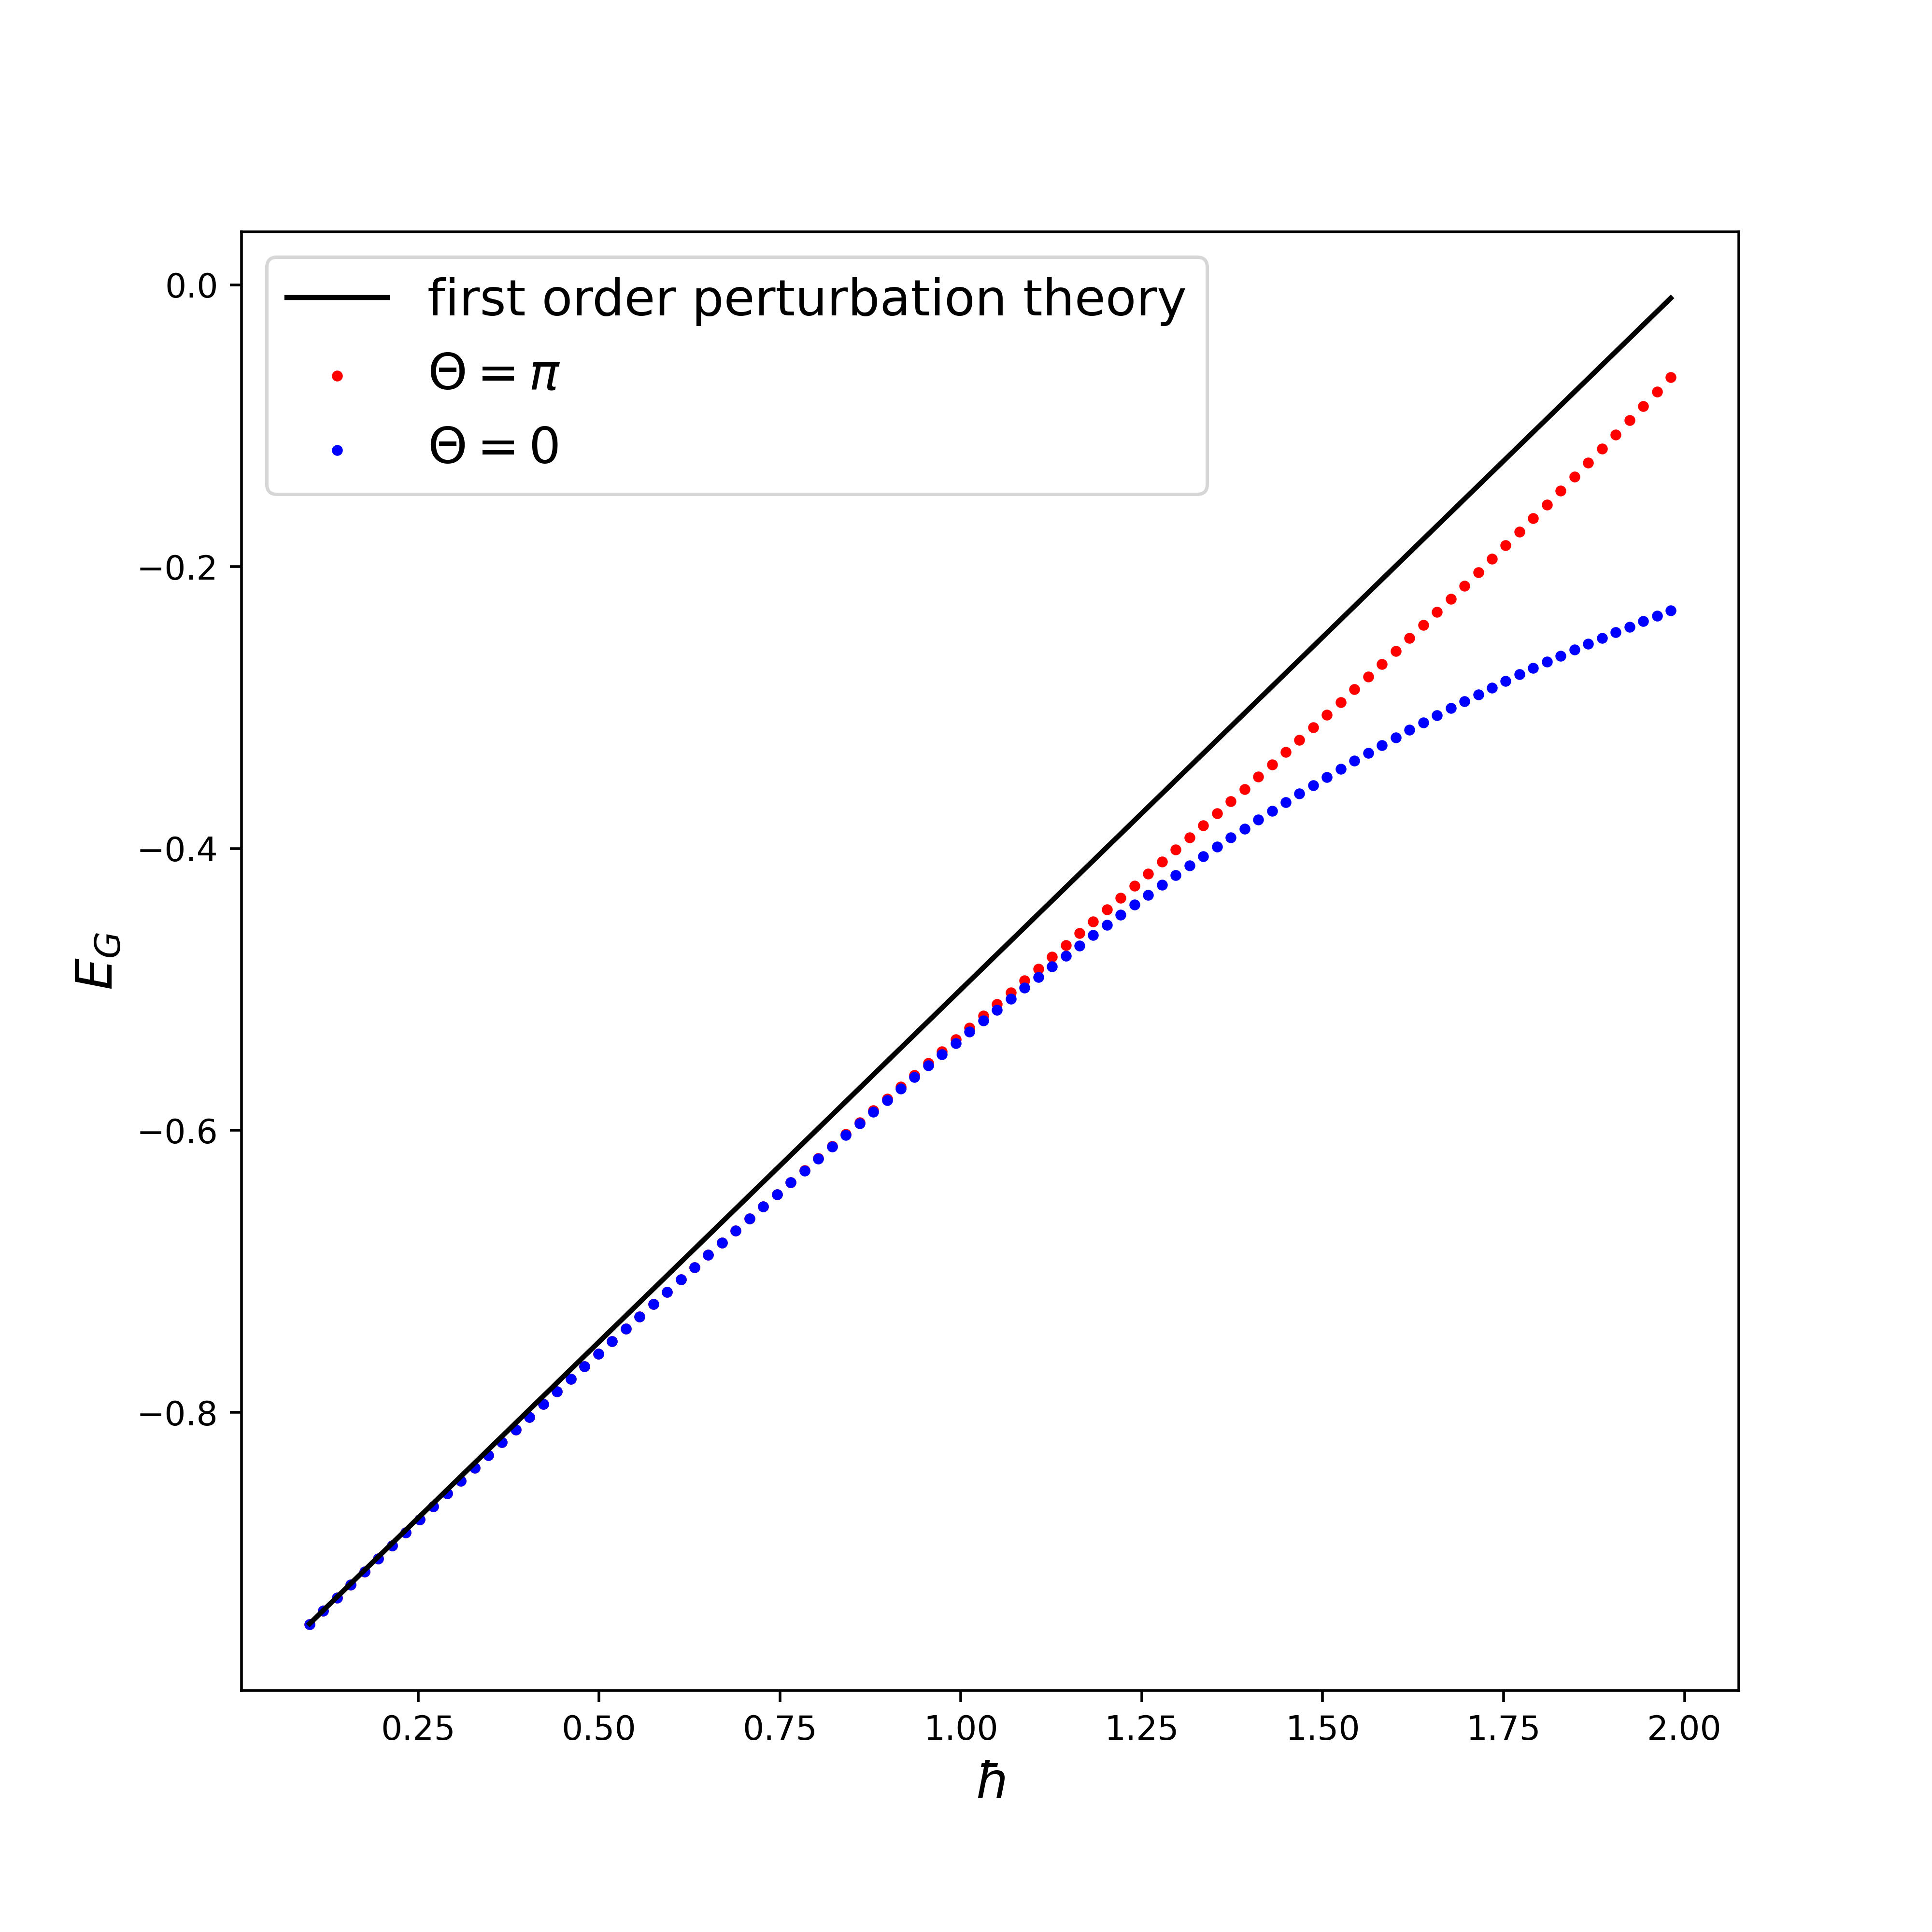
\includegraphics[width=\textwidth]{E_G.png}
        \caption{The ground state energy of the toy model with the $\theta$-term.}
        \label{fig:E_G}
    \end{subfigure}
    \begin{subfigure}{0.5\textwidth}
        \centering
        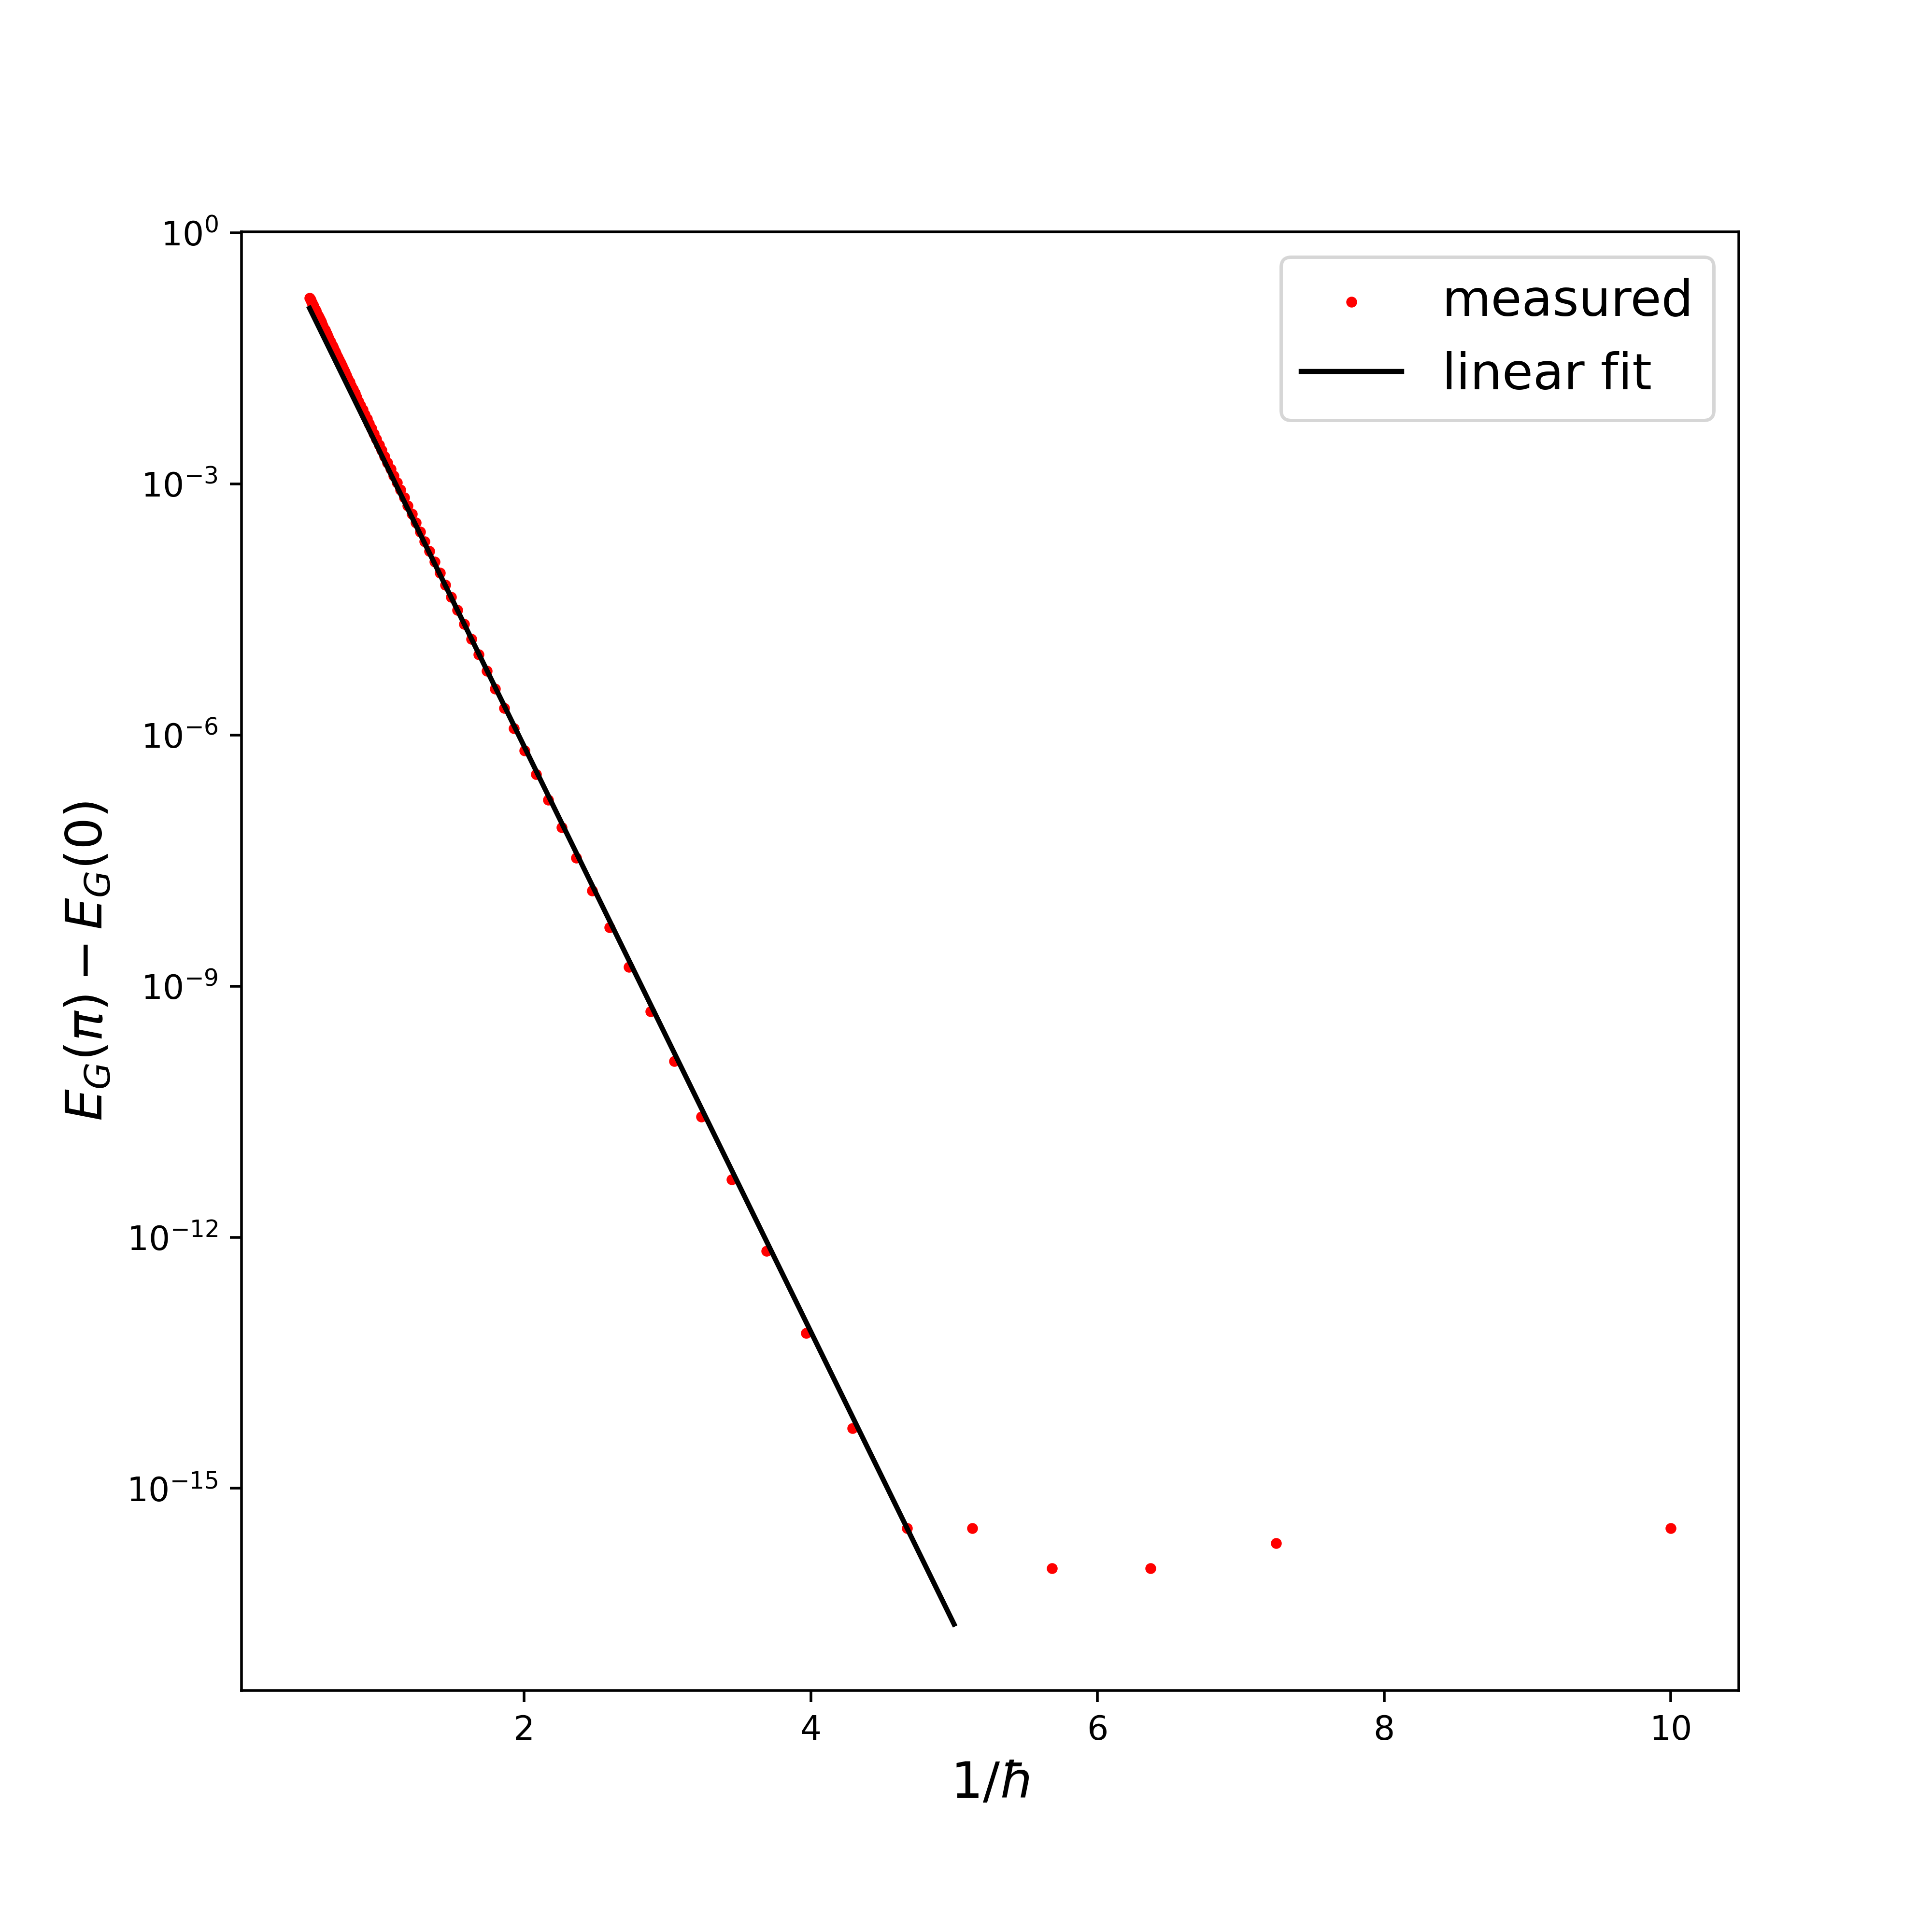
\includegraphics[width=\textwidth]{E_G_diff.png}
        \caption{The difference of the ground state energy with $\theta=0$ and $\theta=\pi$. The slope of the fitting line is $-8.05\pm 0.02$, and this is well matched with the theoretical prediction.}
        \label{fig:E_G_diff}
    \end{subfigure}
\end{figure}

The result shows the ground state energy of the toy model with the $\theta$-term.
In the figure \ref{fig:E_G}, the ground state energy is plotted with $\hbar$.
Here one can see that the difference of two lines supresses very quickly, and this agrees with the theoretical prediction that the $\theta$-term only affects the non-analytic terms in $\hbar$.

The difference of the ground state energy, with $\theta=0$ and $\theta=\pi$ can be calculated as
\[
    E_{gs} = \frac{1}{2}\hbar-2K \cos (\theta ) e^{-S_{\text{inst}}/\hbar}+ \mathcal{O}(\hbar)
\]
\[
    E_{gs}(\theta=\pi)-E_{gs}(\theta=0) = 4K e^{-S_{\text{inst}}/\hbar}
\]
\[
    S_{\text{inst}} = \int_0^{2\pi} dx \sqrt{2(1-\cos x)} = 8
\]
So, the difference of the ground state energy is expected to be
\[
    E_{gs}(\theta=\pi)-E_{gs}(\theta=0) = 4K e^{-S_{\text{inst}}/\hbar} = 4K e^{-8/\hbar}
\]
And this theoretical prediction is well matched with the numerical calculation, as shown in the figure \ref{fig:E_G_diff}.



\subsection{The $\theta$-term in QCD}

In this section, we return to the QCD, and introduce a similar $\theta$-term to the QCD.
The $\theta$-term in QCD is given by
\[
    S_{\theta} = \frac{\theta}{32\pi^2} \int d^4 x \mathrm{tr}(F_{\mu\nu} \tilde{F}^{\mu\nu})
\]
And this action is also a topological, total derivative term, and does not affect the classical EOM.

But, this term affects the quantum theory, by affecting the instanton action.
The instanton action is modified as
\[
    S_{\text{inst}} \rightarrow S_{\text{inst}} + \frac{\theta}{2\pi} \oint d^4 x \mathrm{tr}(F_{\mu\nu} \tilde{F}^{\mu\nu}) = S_{\text{inst}} + \theta n
\]
So this term affects the tunneling amplitude of YM theory, and affects many physical quantities of QCD.
At low energy, QCD coupling constant is large, and it is confinig phase. So there are many non-perturbative(in the coupling constant) effects, and the $\theta$-term can possibly affect all of them.

The $\theta$-dependence of the vacuum energy of QCD is straightforward, just as in the Toy model.
One can calculate the vacuum energy of QCD, with similar calculation using the dilute gas approximation.
\[
    E_{\text{vac}} = E_{\text{vac}}(g) + \Delta(g) \cos(\theta)
\]
Where $E_{\text{vac}}(g)$ is the perturbative part of the vacuum energy, which can be calculated by the perturbation theory, and $\Delta(g)$ is the non-perturbative part of the vacuum energy, which can be calculated by the instanton effect.
The detailed calculation of the vacuum energy of QCD is beyond the scope of this paper, and we will not discuss it here.
One need to consider the instanton moduli space, and the instanton measure, and the instanton determinant, and so on, to calculate the non-perturbative part of the vacuum energy of QCD.

One other important effect of the $\theta$-term is the neutron electric dipole moment.
The $\theta$-term violates the CP symmetry, and this is the only CP-violating term in the QCD.
So all the CP-violating phenomena in the QCD is originated from the $\theta$-term.
The neutron electric dipole moment is a very important physical quantity in this context.
It is a very sensitive probe of the CP violation, so the theoretical prediction of the neutron electric dipole moment is very important to test the QCD and the standard model. 

But the calculation is very complicated, and not based on the path integral formalism. So we will not discuss it here.

\section{Conclusion}

In this paper, we studied the instanton effect in the toy model, and the $\theta$-term in the toy model and QCD.
The instanton effect is a very important non-perturbative effect in the YM theory, and the $\theta$-term is a very important term because it affects all the non-perturbative effects in the QCD.

We introduced the dilute gas approximation to calculate the instanton effect, and showed that the instanton calculation gives the tunneling amplitude, which we cannot obtain by the perturbation theory.
We also showed that this tunneling amplitude equals to the result of the WKB approximation, which is a another non-perturbative method.

Next, we explained the mathematical structure of the YM theory, and the instanton solution, and the instanton moduli space.
The instanton moduli space is the space of the instanton solutions, and calculating the dimension of the instanton moduli space is very important to understand the nature of YM instantons.

After that, we explained the vacuum structure of the YM theory, and the $\theta$-term in the YM theory and QCD.
To explain this, we introduced the quantum mechanics on a circle, and showed that the $\theta$-term affects the non-perturbative part of the ground state energy of the system.
There, we showed the numerical calculation of the ground state energy of the toy model with the $\theta$-term, and showed that the numerical result is well matched with the path integral calulation with dilute gas approximation.

Finally, we explained the neutron electric dipole moment, and the importance of the $\theta$-term in the QCD.






\end{document}

